\chapter{Implementación en simulador}
\label{ch:simulation-implementation}

El entorno de simulación que nos ofrece \ac{sumo} nos permite recoger la práctica totalidad de información propuesta en el capítulo \nameref{ch:methodology} (ver tabla~\ref{tbl:main-variables}) con la excepción del entorno.

El problema es que la representación del entorno que nos ofrece \ac{sumo} está preprocesada, de tal manera que podemos acceder a toda esta información pero de una manera simple. Dicho de otro modo, en un entorno real no podemos saber, por ejemplo, que existe un coche en la posición $(x, y, z)$ de unas determinadas dimensiones\sidenote{
	En realidad sí que podríamos conseguir esa información con cierto grado de certeza, pero existe un porcentaje en el que no, y por tanto necesitamos que ambos entornos sean lo más parecidos posible.
}.

Por lo tanto, la solución por la que se ha optado es por la implementación de un \ac{lidar} en el vehículo simulado de tal manera que ofrece una nube de puntos de las mismas características que las capturadas por el \ac{lidar} físico y situado en la misma posición del vehículo.

\begin{figure}
	\centering
	\subfloat[]{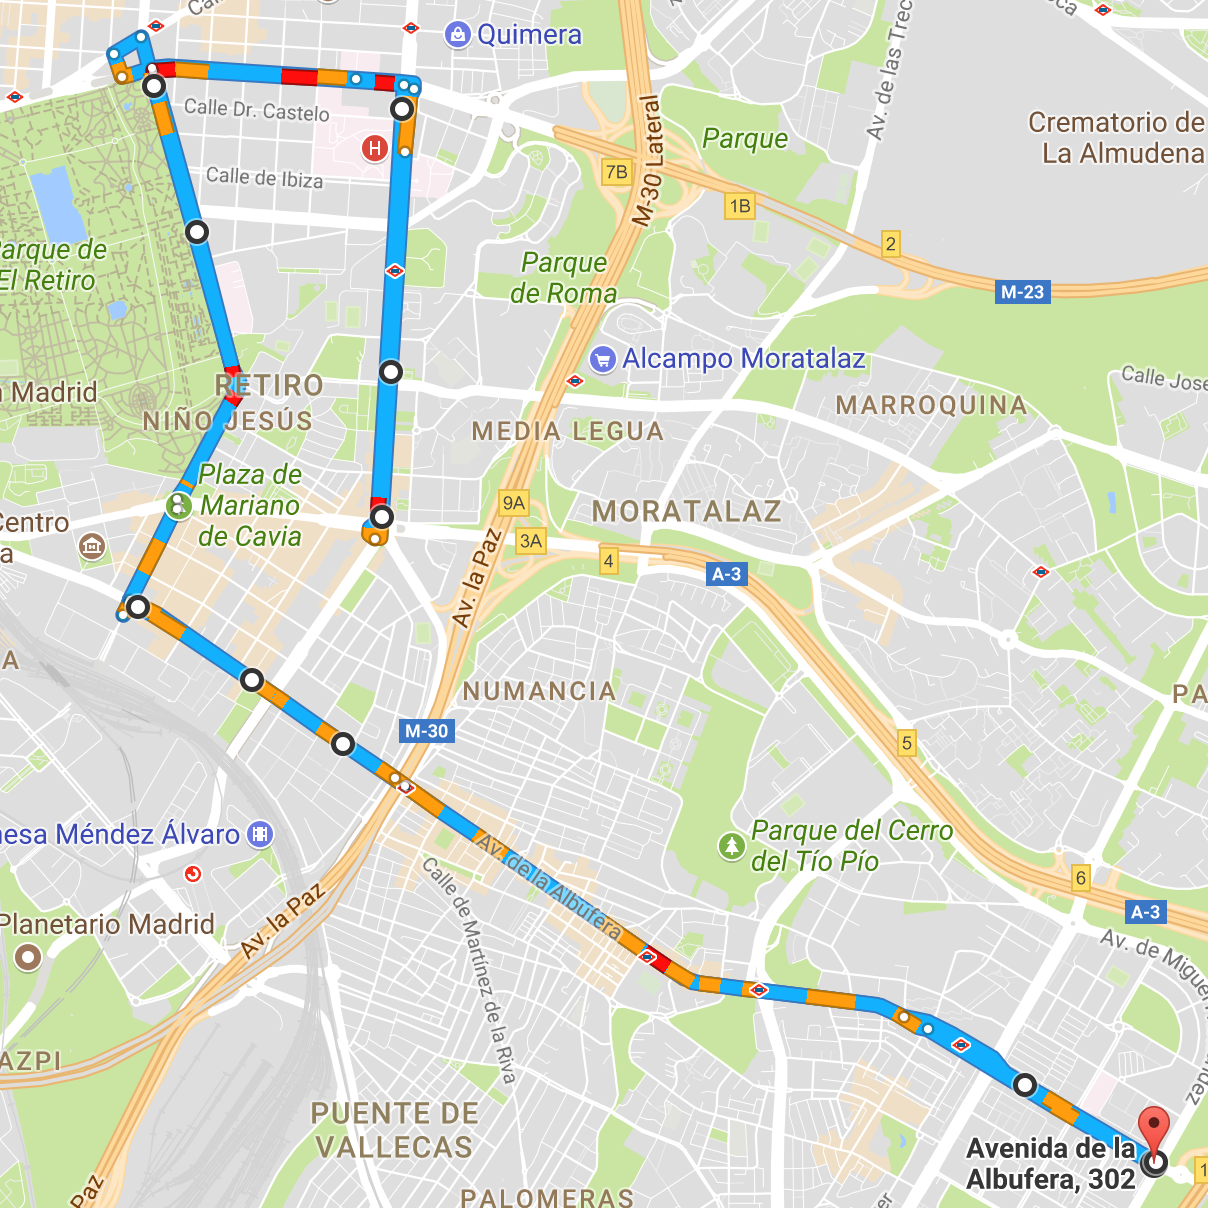
\includegraphics[width=.45\textwidth]{sumo-route-1}}\qquad
	\subfloat[]{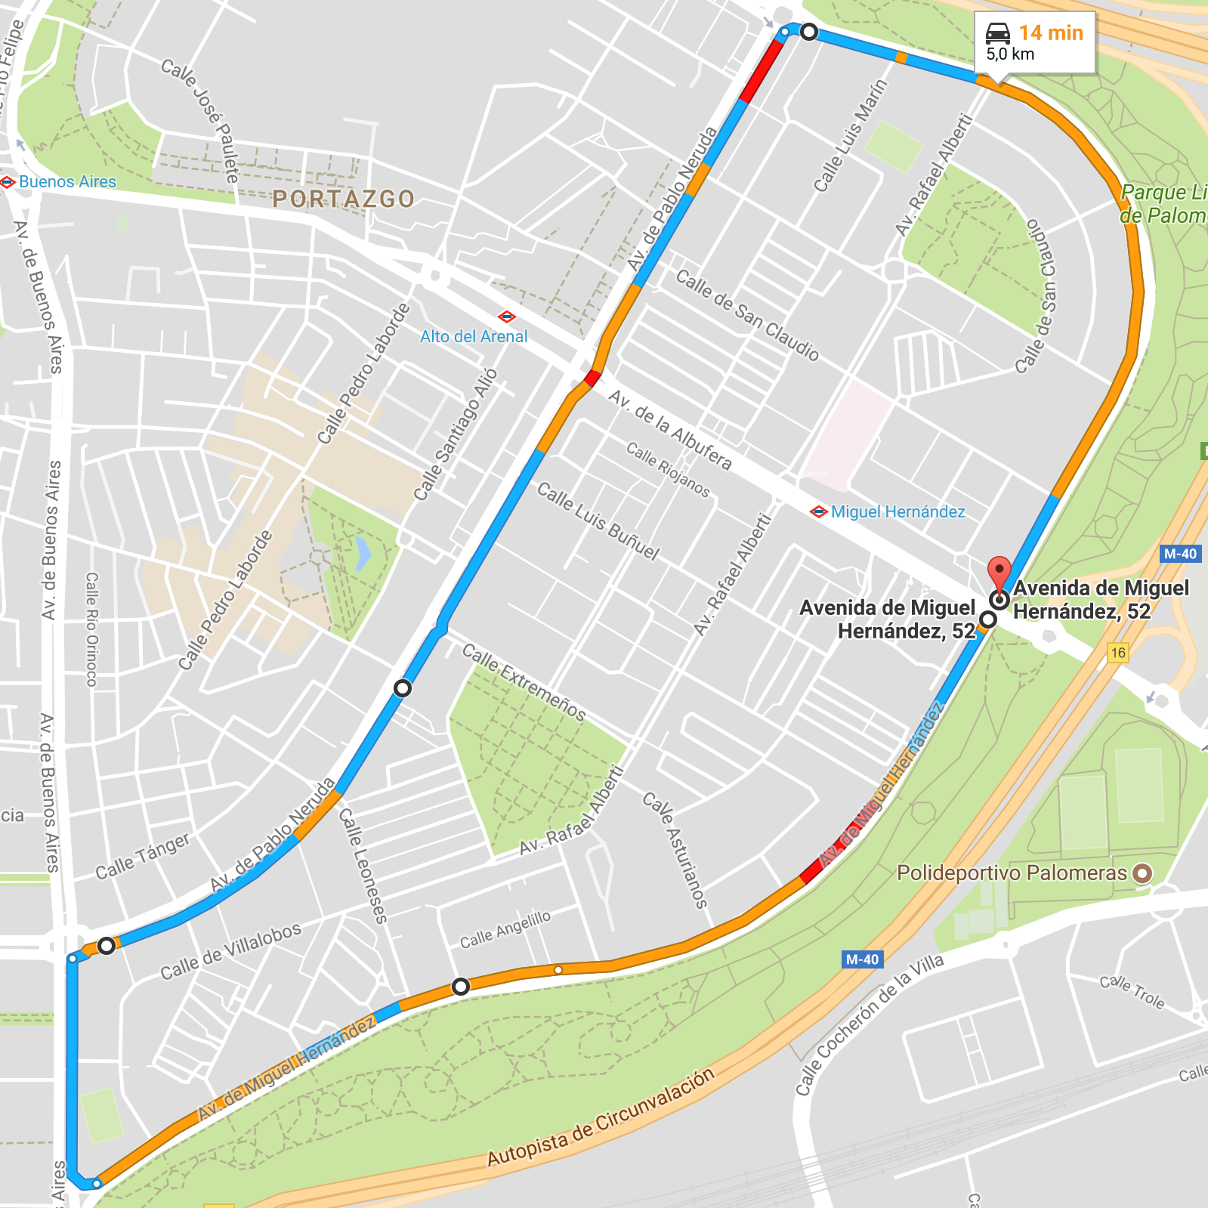
\includegraphics[width=.45\textwidth]{sumo-route-2}}
	\caption[Dos recorridos de prueba en el entorno virtual]{Los dos recorridos generados para recoger los datos de los vehículos circulando con los modelos longitudinal y de cambio de carril implantados.\TODO{Poner la ruta de verdad}}
	\label{fig:sumo-routes}
\end{figure}

Una vez implementado el vehículo, dentro de la librería desarrollada se han implantado los modelos longitudinales y de cambio de carril dentro de un conductor virtual para el sujeto global y para cada uno de los sujetos del experimento y se han realizado dos recorridos de características similares a los recorridos de los que se han obtenido los conjuntos de test (ver Figura~\ref{fig:sumo-routes}).

La forma propuesta para comprobar si los comportamientos son similares es hacer un cálculo de los indicadores propuestos en~\cite{DiazAlvarez2014} para el comportamiento longitudinal, y de la media de cambios de carril por tiempo de recorrido para el modelo de cambio de carril. En la tabla~\ref{tbl:global-comparison-indicators} se resumen estos valores para el modelo de conducción global y los conductores específicos. La leyenda de indicadores es la siguiente:

\begin{itemize}
	\item $V$. Velocidad instantánea del vehículo.
	\item $AP$/$AN$. Aceleración instantánea positiva y negativa del vehículo.
	\item $JIM$. Jerk\sidenote{El \textbf{jerk} es la derivada de la aceleración.} positivo con aceleración positiva, el cual se corresponde con la situación en la que el vehículo está iniciando la marcha (jerk de inicio de marcha).
	\item $JLC$. Jerk positivo con aceleración negativa, caso que se da cuando se está llegando a la velocidad deseada, por lo que aunque la velocidad sigue aumentando, lo hace en una tasa cada vez más decreciente (jerk de llegada a crucero).
	\item $JIF$. Jerk negativo con aceleración negativa, cuando el conductor inicia una maniobra de reducción de velocidad (jerk de inicio de frenada).
	\item $JFF$. Jerk positivo con aceleración negativa, que se corresponde con el moento en el que el conductor está terminando una manibra de frenada o de reducción de velocidad (jerk de fin de frenada).
\end{itemize}

\begin{table*}
	\centering
	\caption[Indicadores reales frente a indicadores capturados en simulación]{Resumen de los indicadores provenientes de los datos de los conductores en los recorridos frente a los valores.}
	\label{tbl:global-comparison-indicators}
	\begin{tabular}{cccccccccc}
		\multicolumn{2}{c}{}                   & \multicolumn{2}{c}{\textbf{$S_1$}}    & \multicolumn{2}{c}{\textbf{$S_1$}}          & \multicolumn{2}{c}{\textbf{$S_2$}}        & \multicolumn{2}{c}{\textbf{$S_3$}}        \\
		\multicolumn{2}{l}{}                   & $\mu$                      & $\sigma$ & $\mu$                            & $\sigma$ & $\mu$                          & $\sigma$ & $\mu$                          & $\sigma$ \\
		\multirow{2}{*}{\textbf{$V$}}   & Real & \multicolumn{1}{c}{$X.XX$} & $X.XX$   & \multicolumn{1}{c}{$0.059783$}   & $X.XX$   & \multicolumn{1}{c}{$0.072001$} & $X.XX$   & \multicolumn{1}{c}{$0.070744$} & $X.XX$   \\
		& Sim  &                            &          &                                  &          &                                &          &                                &          \\
		\multirow{2}{*}{\textbf{$AP$}}  & Real & \multicolumn{1}{c}{$X.XX$} & $X.XX$   & \multicolumn{1}{c}{\$\$0.209081} & $X.XX$   & \multicolumn{1}{c}{$0.20866$}  & $X.XX$   & \multicolumn{1}{c}{$0.213288$} & $X.XX$   \\
		& Sim  &                            &          &                                  &          &                                &          &                                &          \\
		\multirow{2}{*}{\textbf{$AN$}}  & Real & \multicolumn{1}{c}{$X.XX$} & $X.XX$   & \multicolumn{1}{c}{$0.065544$}   & $X.XX$   & \multicolumn{1}{c}{$0.066772$} & $X.XX$   & \multicolumn{1}{c}{$0.057586$} & $X.XX$   \\
		& Sim  &                            &          &                                  &          &                                &          &                                &          \\
		\multirow{2}{*}{\textbf{$JIM$}} & Real & \multicolumn{1}{c}{$X.XX$} & $X.XX$   & \multicolumn{1}{c}{$X.XX$}       & $X.XX$   & \multicolumn{1}{c}{$X.XX$}     & $X.XX$   & \multicolumn{1}{c}{$X.XX$}     & $X.XX$   \\
		& Sim  &                            &          &                                  &          &                                &          &                                &          \\
		\multirow{2}{*}{\textbf{$JLC$}} & Real & \multicolumn{1}{c}{$X.XX$} & $X.XX$   & \multicolumn{1}{c}{$X.XX$}       & $X.XX$   & \multicolumn{1}{c}{$X.XX$}     & $X.XX$   & \multicolumn{1}{c}{$X.XX$}     & $X.XX$   \\
		& Sim  &                            &          &                                  &          &                                &          &                                &          \\
		\multirow{2}{*}{\textbf{$JIF$}} & Real & \multicolumn{1}{c}{$X.XX$} & $X.XX$   & \multicolumn{1}{c}{$X.XX$}       & $X.XX$   & \multicolumn{1}{c}{$X.XX$}     & $X.XX$   & \multicolumn{1}{c}{$X.XX$}     & $X.XX$   \\
		& Sim  &                            &          &                                  &          &                                &          &                                &          \\
		\multirow{2}{*}{\textbf{$JFF$}} & Real & \multicolumn{1}{c}{$X.XX$} & $X.XX$   & \multicolumn{1}{c}{$X.XX$}       & $X.XX$   & \multicolumn{1}{c}{$X.XX$}     & $X.XX$   & \multicolumn{1}{c}{$X.XX$}     & $X.XX$   \\
		& Sim  &                            &          &                                  &          &                                &          &                                &          \\
		\multirow{2}{*}{\textbf{$MCC$}} & Real & \multicolumn{1}{c}{$X.XX$} & $X.XX$   & \multicolumn{1}{c}{$X.XX$}       & $X.XX$   & \multicolumn{1}{c}{$X.XX$}     & $X.XX$   & \multicolumn{1}{c}{$X.XX$}     & $X.XX$   \\
		& Sim  &                            &          &                                  &          &                                &          &                                &         
	\end{tabular}
\end{table*}

La tabla~\ref{tbl:global-comparison-indicators} ofrece mucha información, por lo que la comentaremos por partes.

\section{Comportamiento en modelo de conductor general}

\TODO{Comentar cuando tengamos la tabla rellena}

\section{Comportamiento en modelos de conductor específicos}

\TODO{Comentar cuando tengamos la tabla rellena}

\section{Validación del modelo}

